\testfile{pgfplotstest.align.tex}
\testsection{Anchors, alignment, baselines, sub nodes}%
\testsubsection{Baseline alignment}
\noindent
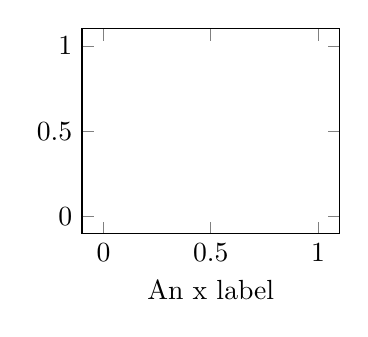
\begin{tikzpicture}[baseline]
	\begin{axis}[width=0.4\linewidth,xlabel=An x label]
		\smallplotstest
	\end{axis}
\end{tikzpicture}
\hspace{1cm}
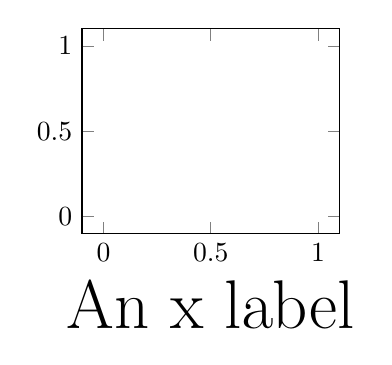
\begin{tikzpicture}[baseline]
	\begin{axis}[width=0.4\linewidth,xlabel={\Huge An x label}]
		\smallplotstest
	\end{axis}
\end{tikzpicture}

\testsubsection{Baseline alignment and externalized graphics}
One needs \texttt{\textbackslash beginpgfgraphicnamed} around the complete paragraph, so this here doesn't work (see source code):

\beginpgfgraphicnamed{baselinetesta}
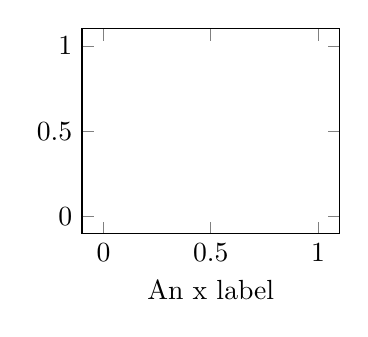
\begin{tikzpicture}[baseline]
\begin{axis}[width=0.4\linewidth,xlabel=An x label]
	\smallplotstest
\end{axis}
\end{tikzpicture}
\endpgfgraphicnamed
%
%
\hspace{1cm}
\beginpgfgraphicnamed{baselinetestb}
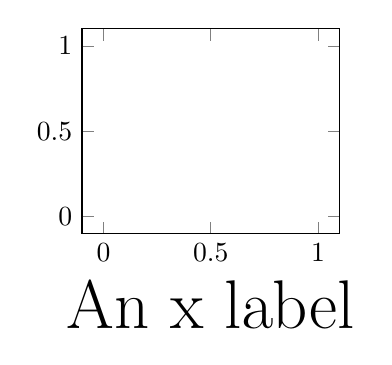
\begin{tikzpicture}[baseline]
\begin{axis}[width=0.4\linewidth,xlabel={\Huge An x label}]
	\smallplotstest
\end{axis}
\end{tikzpicture}
\endpgfgraphicnamed

\testsubsection{Baseline alignment and externalized graphics II}
\beginpgfgraphicnamed{baselinetestc}
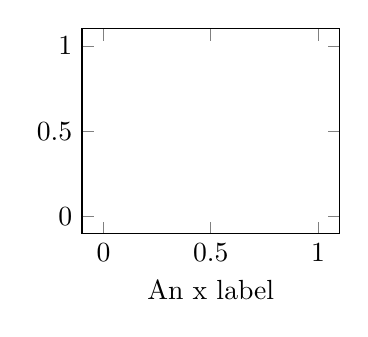
\begin{tikzpicture}[baseline]
\begin{axis}[width=0.4\linewidth,xlabel=An x label]
	\smallplotstest
\end{axis}
\end{tikzpicture}
%
%
\hspace{1cm}
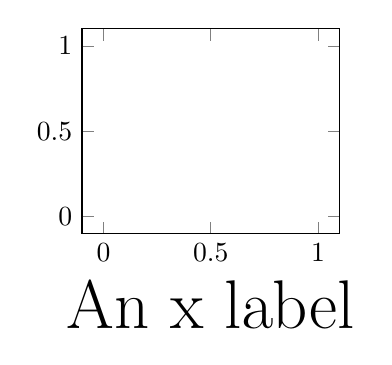
\begin{tikzpicture}[baseline]
\begin{axis}[width=0.4\linewidth,xlabel={\Huge An x label}]
	\smallplotstest
\end{axis}
\end{tikzpicture}
\endpgfgraphicnamed

\testsubsection{Horizontal and Vertical alignment}
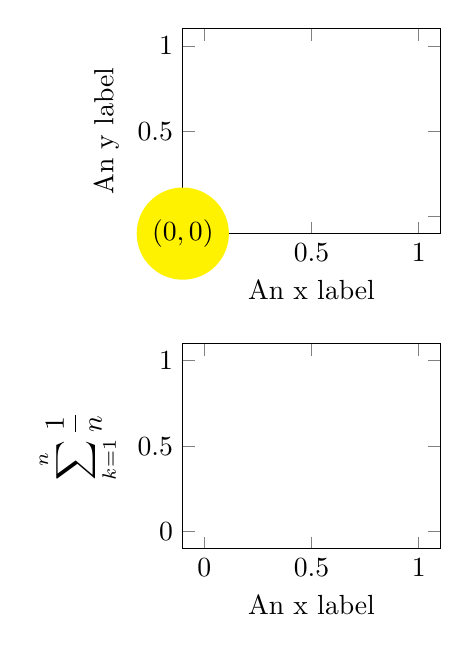
\begin{tikzpicture}[baseline]
\begin{axis}[width=0.4\linewidth,xlabel=An x label,ylabel=An y label]
	\smallplotstest
\end{axis}

\begin{scope}[yshift=-4cm]
\begin{axis}[width=0.4\linewidth,xlabel=An x label,ylabel={$\displaystyle\sum_{k=1}^n \frac 1n$}]
	\smallplotstest
\end{axis}
\end{scope}

\node[fill=yellow,circle] at (0,0) {$(0,0)$};
\end{tikzpicture}
%
%
\hspace{1cm}
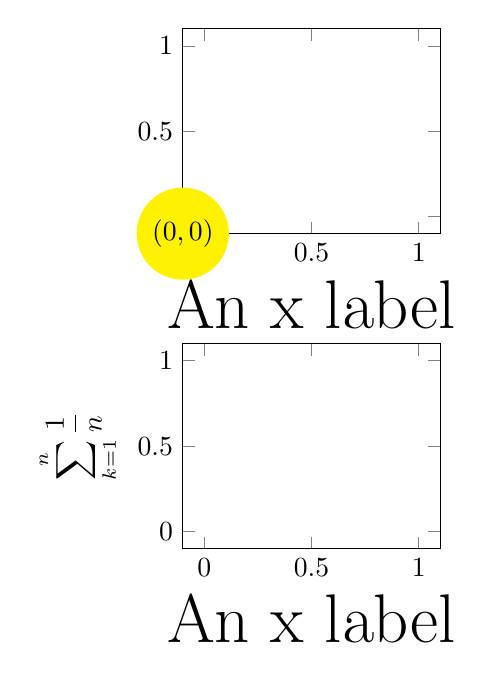
\begin{tikzpicture}[baseline]
\begin{axis}[width=0.4\linewidth,xlabel={\Huge An x label}]
	\smallplotstest
\end{axis}

\begin{scope}[yshift=-4cm]
\begin{axis}[width=0.4\linewidth,xlabel={\Huge An x label},ylabel={$\displaystyle\sum_{k=1}^n \frac 1n$}]
	\smallplotstest
\end{axis}
\end{scope}
\node[fill=yellow,circle] at (0,0) {$(0,0)$};
\end{tikzpicture}

\testsubsection{Anchortest}
{
\setlength{\fboxsep}{0pt}%
\def\showanchorplot#1{%
	\begin{axis}[
		width=5cm,
		anchor=#1,
		title=My title,
		xlabel=$x$,
		ylabel=$y$
	]
		\smallplotstest
		\addlegendentry{My plot}
	\end{axis}
}%
\def\showanchor#1{
	\vbox{\hsize=5cm
	#1:

	\pgfplotsset{every axis legend/.append style={at={(1.03,1)},anchor=north west}}
	\fbox{%
	\begin{tikzpicture}
		\showanchorplot{#1}%
		\begin{pgfinterruptboundingbox}
		\node[fill=yellow,circle] at (0,0) {$(0,0)$};
		\end{pgfinterruptboundingbox}
	\end{tikzpicture}
	}%
	}
}%
\showanchor{outer center}
\showanchor{outer north}
\showanchor{outer north east}
\showanchor{outer east}
\showanchor{outer south east}
\showanchor{outer south}
\showanchor{outer south west}
\showanchor{outer west}
\showanchor{outer north west}
\showanchor{center}
\showanchor{north}
\showanchor{north east}
\showanchor{east}
\showanchor{south east}
\showanchor{south}
\showanchor{south west}
\showanchor{west}
\showanchor{north west}
\showanchor{above north}
\showanchor{above north east}
\showanchor{right of north east}
\showanchor{right of east}
\showanchor{right of south east}
\showanchor{below south east}
\showanchor{below south}
\showanchor{below south west}
\showanchor{left of south west}
\showanchor{left of west}
\showanchor{left of north west}
\showanchor{above north west}
\showanchor{above north west}
\showanchor{origin}
\showanchor{above origin}
\showanchor{right of origin}
\showanchor{below origin}
\showanchor{left of origin}

\def\showanchorplot#1{%
	\begin{axis}[
		width=5cm,
		anchor=#1,
		title=My title,
		xlabel=$x$,
		ylabel=$y$,
		axis x line=center,axis y line=center,
		tick align=center,
	]
		\addplot plot[domain=-2:10] (\x,5*\x);
		\addlegendentry{My plot}
	\end{axis}
}%
\showanchor{origin}
\showanchor{above origin}
\showanchor{right of origin}
\showanchor{below origin}
\showanchor{left of origin}
}


\testsubsection{Accessing sub-nodes}
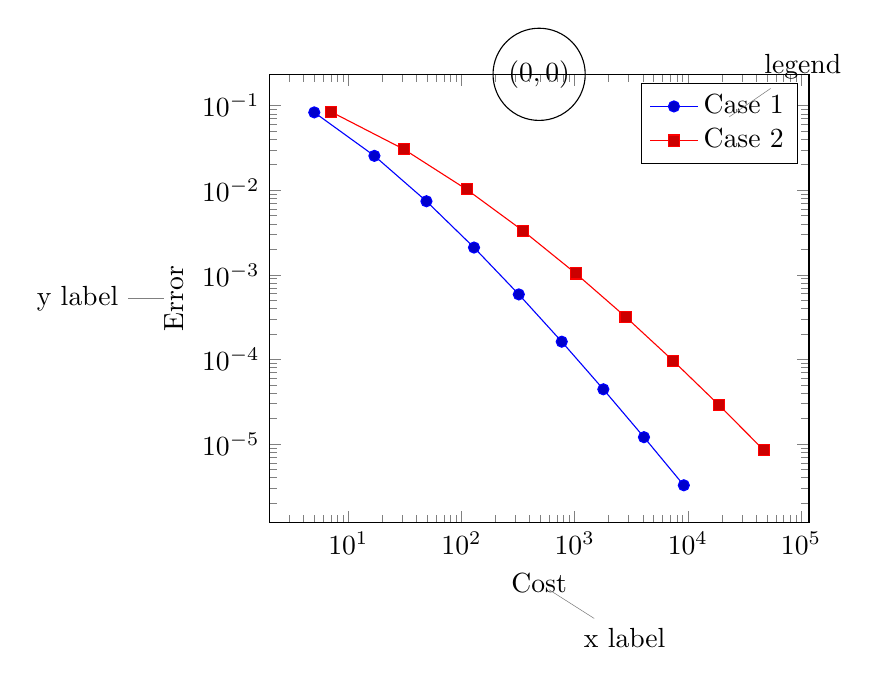
\begin{tikzpicture}[baseline]%
	\node[circle,draw=black] at (0,0) {$(0,0)$};
	\begin{loglogaxis}[
		anchor=north,
		name=firstplot,
		xlabel=Cost,
		ylabel=Error,
		y label style={name=myylabel},
		x label style={name=myxlabel},
		legend style={name=mylegend,
			row 1 column 2/.style={blue,name=firstentry}% doesn't work!
		}
	]
	\addplot plot coordinates {
		(5,     8.31160034e-02)
		(17,    2.54685628e-02)
		(49,    7.40715288e-03)
		(129,   2.10192154e-03)
		(321,   5.87352989e-04)
		(769,   1.62269942e-04)
		(1793, 4.44248889e-05)
		(4097, 1.20714122e-05)
		(9217, 3.26101452e-06)
	};
	\addplot plot coordinates {
		(7,     8.47178381e-02)
		(31,    3.04409349e-02)
		(111,   1.02214539e-02)
		(351,   3.30346265e-03)
		(1023,  1.03886535e-03)
		(2815,  3.19646457e-04)
		(7423,  9.65789766e-05)
		(18943, 2.87339125e-05)
		(47103, 8.43749881e-06)
	};
	\legend{Case 1\\Case 2\\}
	\end{loglogaxis}

	\node[pin=45:legend] at (mylegend.center) {};
	\node[pin=-45:x label] at (myxlabel.center) {};
	\node[pin=180:y label] at (myylabel.center) {};
\end{tikzpicture}%

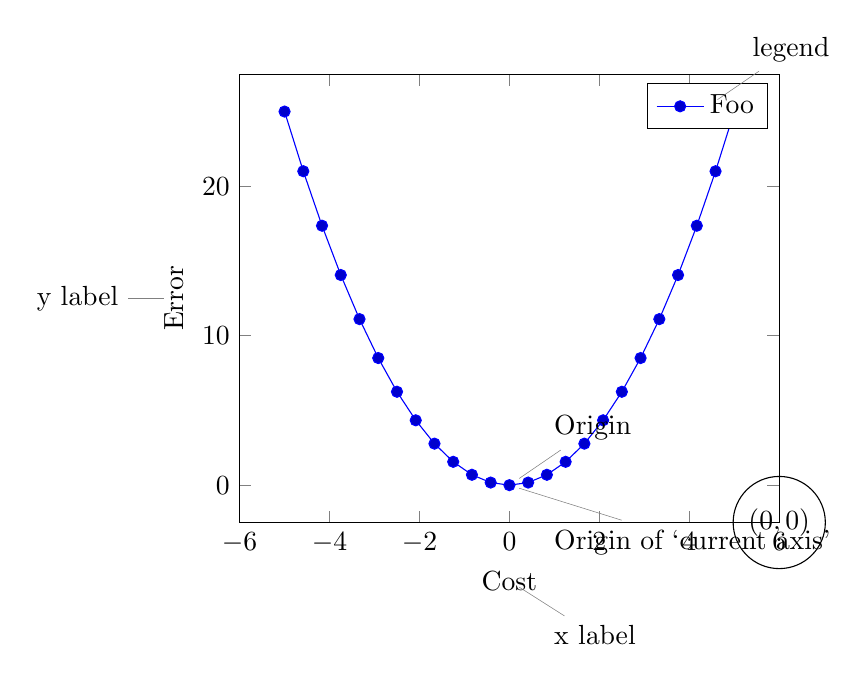
\begin{tikzpicture}[baseline]%
	\node[circle,draw=black] at (0,0) {$(0,0)$};
	\begin{axis}[
		anchor=south east,
		name=firstplot,
		xlabel=Cost,
		ylabel=Error,
		y label style={name=myylabel},
		x label style={name=myxlabel},
		legend style={name=mylegend,
			row 1 column 2/.style={blue,name=firstentry}% doesn't work!
		}
	]
	\addplot (\x,\x^2);
	\legend{Foo}
	\end{axis}

	\node[pin=45:legend] at (mylegend.center) {};
	\node[pin=-45:x label] at (myxlabel.center) {};
	\node[pin=180:y label] at (myylabel.center) {};

	\node[pin=45:Origin] at (firstplot.origin) {};
	\node[pin=-45:Origin of `current axis'] at (current axis.origin) {};
\end{tikzpicture}%


\testsubsection{Funny bounding boxes}
\testsubsubsection{(my plot.below south west) rectangle (my plot.above north east)}
{
The following figure is centered:
\setlength{\fboxsep}{0pt}%
\begin{center}
\fbox{%
\begin{tikzpicture}%
	\begin{pgfinterruptboundingbox}
	\pgfplotsset{every axis legend/.append style={at={(1.03,1)},anchor=north west}}
	\begin{axis}[
		name=my plot,
		title=A title,
		xlabel={\Huge An x label},
		ylabel={$\displaystyle\sum_{k=1}^n \frac 1n$}
	]
		\smallplotstest
		\addlegendentry{My plot}
	\end{axis}
	\end{pgfinterruptboundingbox}

	\useasboundingbox (my plot.below south west) rectangle (my plot.above north east);
\end{tikzpicture}%
}%
\end{center}
}
